\documentclass[tikz,border=10pt]{standalone}
% Adicione 'fit' e 'backgrounds' (opcional, mas recomendado)
\usetikzlibrary{positioning, arrows.meta, fit, backgrounds}

\begin{document}
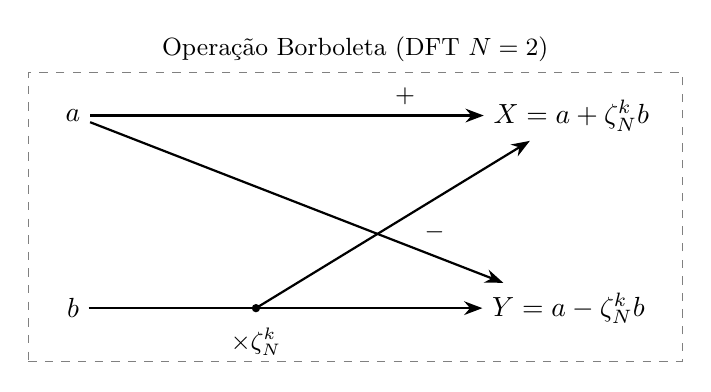
\begin{tikzpicture}[
    node distance=2cm and 3cm,
    dot/.style={circle, fill, inner sep=1.5pt},
    arrow/.style={-Stealth, thick}
]

    % Entradas
    \node (in1) {$a$};
    \node (in2) [below=of in1] {$b$};

    % Pontos de junção/multiplicação
    \node (mid) [right=of in2, xshift=-1cm, label=below:{\small $\times \zeta_N^k$}] {};
    \fill (in2 -| mid) circle (1.5pt) coordinate (mult);

    % Saídas
    \node (out1) [right=of in1, xshift=2cm] {$X = a + \zeta_N^k b$};
    \node (out2) [right=of in2, xshift=2cm] {$Y = a - \zeta_N^k b$};

    % Linhas e Conexões
    \draw[arrow] (in1) -- (out1) node[pos=0.8, above] {\small $+$};
    \draw[arrow] (in1) -- (out2) node[pos=0.8, xshift=5pt, above] {\small $-$};
    
    \draw[thick] (in2) -- (mult);
    \draw[arrow] (mult) -- (out1);
    \draw[arrow] (mult) -- (out2);

    % O RETÂNGULO QUE ESTAVA DANDO ERRO:
    % Agora o TikZ reconhecerá a chave 'fit'
    \node[draw, dashed, gray, fit=(in1) (out2), inner sep=10pt, label=above:{\small Operação Borboleta (DFT $N=2$)}] {};

\end{tikzpicture}
\end{document}